\documentclass[12pt,a4paper,english,firamath]{nsi}
\pagestyle{empty}

\begin{document}
\titre{Evaluation Chart}
\classe{Euro 1\ere}
\maketitle

Élève évalué\cdot e : \dotfill\\


Élève correcteur\cdot trice : \dotfill\\



\begin{center}
    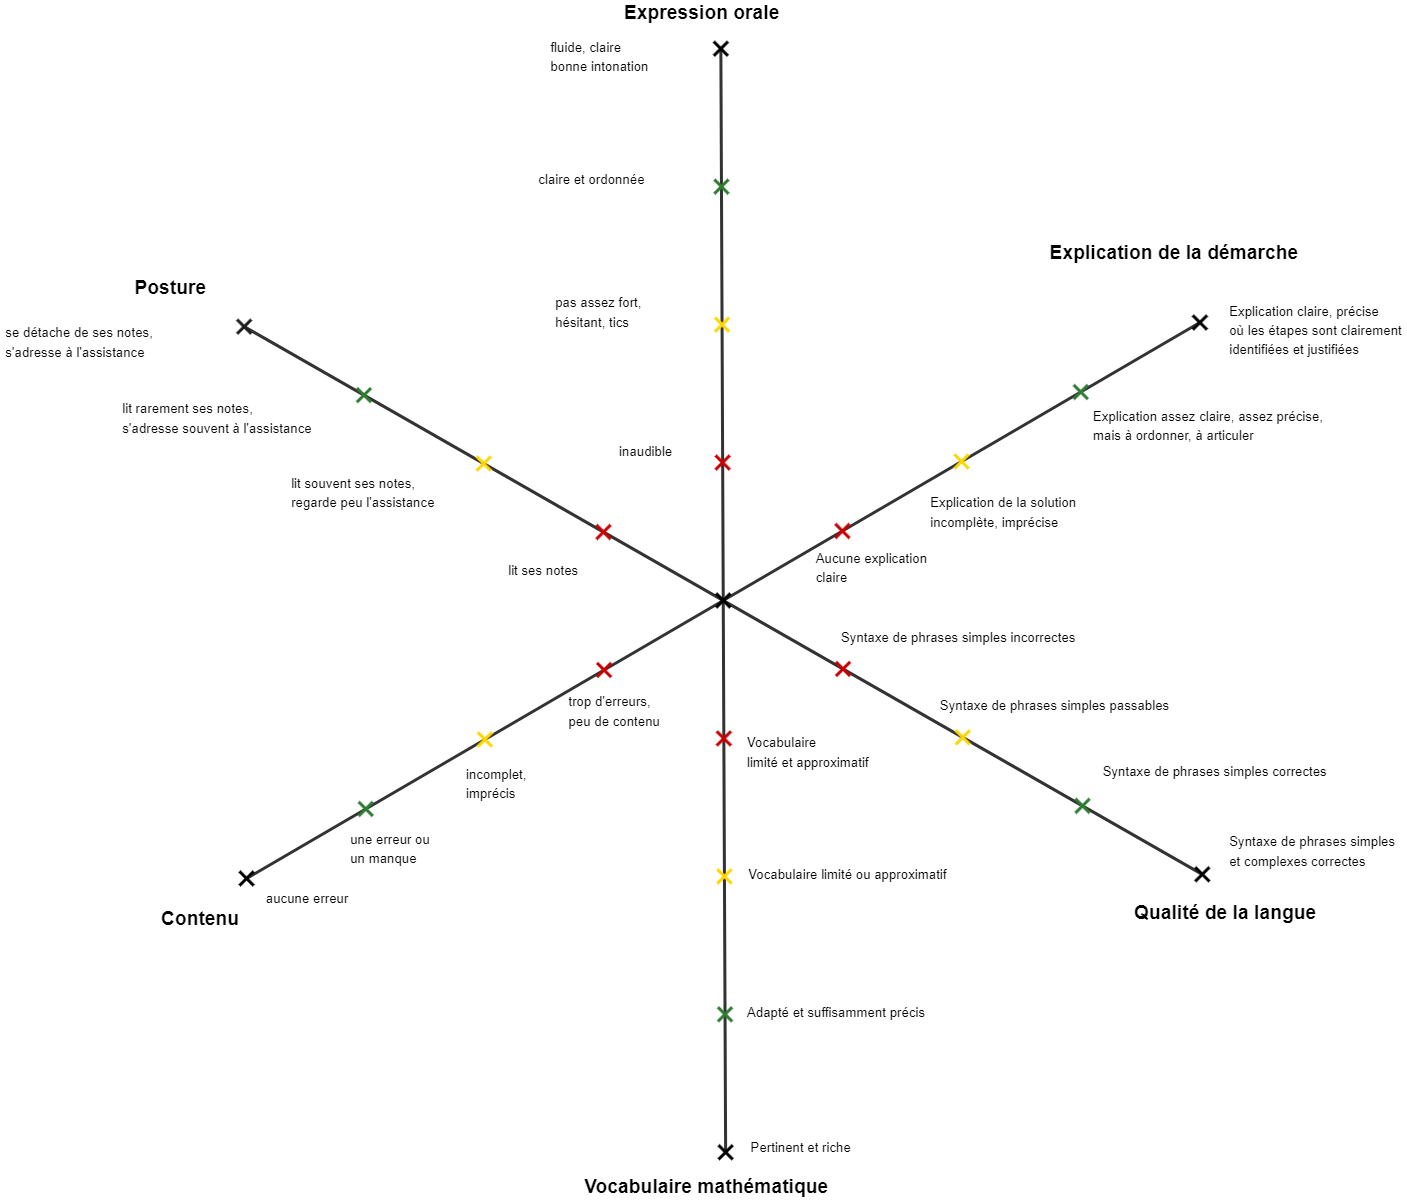
\includegraphics[width=16cm]{img/grid.png}
\end{center}
\begin{multicols}{2}
    Points forts :\\[.5em]
    \carreauxseyes{8}{4.8}
    \columnbreak
    
    Conseils :\\[.5em]
    \carreauxseyes{8}{4.8}
\end{multicols}
\end{document}